\documentclass{standalone}
\usepackage{tikz}


\begin{document}

\begin{tikzpicture}
	\node[inner sep=0] (N) at (0, 0) {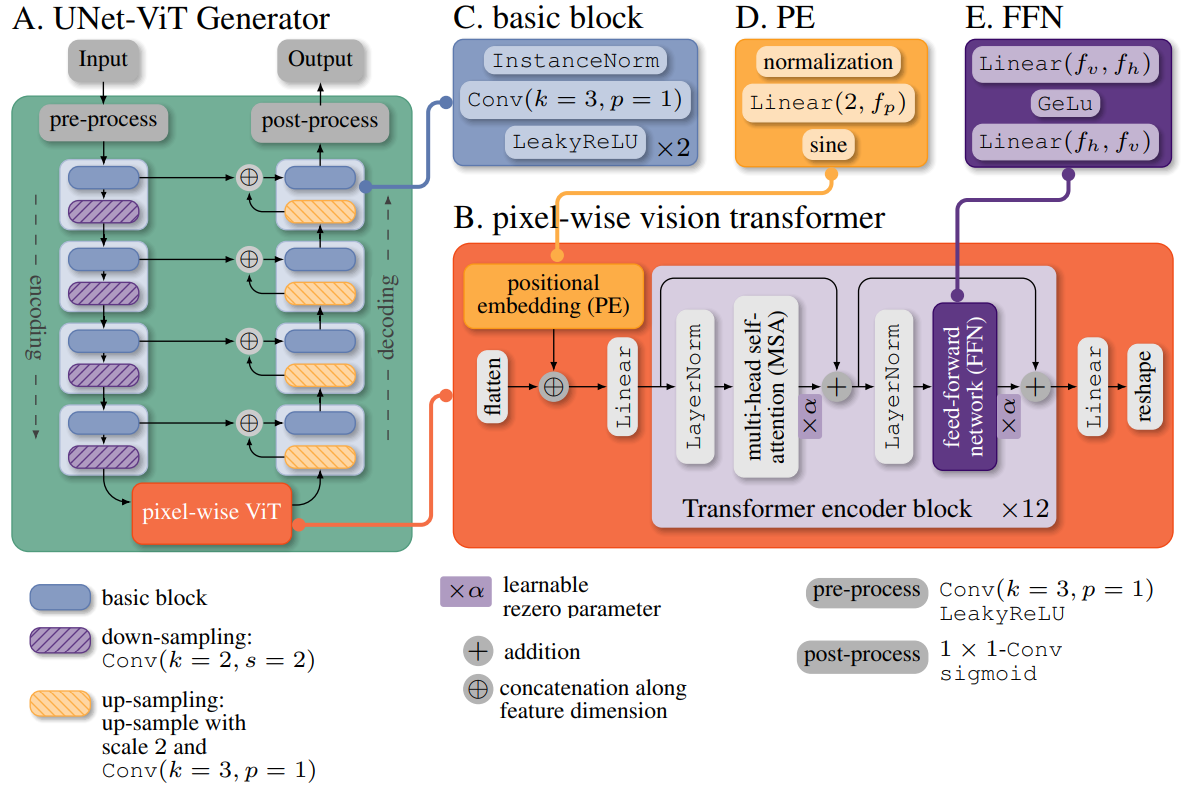
\includegraphics[height=13.5cm]{network.png}};
	\node[inner sep=0, anchor=north west] (S1) at (N.north east) {\includegraphics[height=13.5cm]{supplementary_anime.png}};
	\node[inner sep=0, anchor=north west] (S2) at ([xshift=.15cm]S1.north east) {\includegraphics[height=13.5cm]{supplementary_gender.png}};
	\node[inner sep=0, anchor=north west] (S3) at ([xshift=.15cm]S2.north east) {\includegraphics[height=13.5cm]{supplementary_glasses.png}};
\end{tikzpicture}

\end{document}